\section{Counting the ranks}\label{sec:count}

Recall that
\[
D_q(t)=1-t-t^3-\dots-t^{2q-3},\qquad
R_q(t)=1+t^2+\dots+t^{2q-6},\qquad
N_q(t)=1+t^2+\dots+t^{2q-4}-t^{2q-3},
\]
with $R_3=1$. Note that $t^3R_q(t)=t^3+t^5+\dots+t^{2q-3}$, so $D_q=1-t-t^3R_q$.

\begin{theorem}[Theorem~A$_q$]\label{thm:Aq}
Let $q\ge3$. Then
\[
\sum_{n\ge1}r_q(n)\,t^n=\frac{t\,R_q(t)}{D_q(t)},\qquad \sum_{n\ge0}a_q(n)\,t^n=\frac{N_q(t)}{D_q(t)},
\]
$a_q(0)=1$ and $a_q(n)=r_q(n)+r_q(n-1)$ for $n\ge1$,
and $\gcd(N_q,D_q)=1$. Hence $a_q(n)=a_q(n-1)+a_q(n-3)+\dots+a_q(n-2q+3)$ for every $n\ge2q-2$, and at
$n=2q-3$ the left side minus the right side is $-1$. For $m=1,2,3$ these are the counts of the
rationals of rank $n$ in the $m$-tree.
\end{theorem}

\begin{proof}
\emph{Positive points.} By Theorem~\ref{thm:Bq}, $r_q(n)$ is the number of strings with $c_1\ge1$,
$c_2,\dots,c_k\ge1$, no run of more than $q-3$ ones among $c_2,\dots,c_k$, and weight $n$. Give $c_1$
the weight $c_1$ and each $c_j$ with $j\ge2$ the weight $c_j+1$, which counts the $g$ next to it. Then
$c_1$ contributes $t/(1-t)$, a later digit $1$ contributes $u=t^2$, and a later digit at least $2$
contributes $B=\sum_{c\ge2}t^{c+1}=t^3/(1-t)$. Read from left to right, the sequence $c_2,\dots,c_k$ is
in exactly one way a run of at most $q-3$ ones followed by some number of blocks, where each block is
one digit at least $2$ followed by a run of at most $q-3$ ones. A run contributes
$1+u+\dots+u^{q-3}=R_q(t)$. So
\[
\sum_{n\ge1}r_q(n)\,t^n=\frac{t}{1-t}\cdot R_q\cdot\frac{1}{1-BR_q}=\frac{tR_q}{(1-t)(1-BR_q)}=\frac{tR_q}{1-t-t^3R_q}
=\frac{tR_q}{D_q}.
\]
The geometric series makes sense as a formal power series because $B$ has no constant term.

\emph{Negative points.} By (D2) and (D3), $X\mapsto-1/X$ is a bijection from the negative points of
rank $n$ onto the positive points of rank $n-1$. Every point of rank $n\ge1$ is nonzero, so
$a_q(n)=r_q(n)+r_q(n-1)$. Hence
\[
\sum_{n\ge0}a_q(n)\,t^n=1+(1+t)\frac{tR_q}{D_q}=\frac{D_q+(t+t^2+t^3+\dots+t^{2q-4})}{D_q}=\frac{N_q}{D_q},
\]
since $(1+t)tR_q=t+t^2+\dots+t^{2q-4}$, and adding this to $D_q$ cancels $t,t^3,\dots,t^{2q-5}$.

\emph{Lowest terms.} Let $\alpha$ be a common complex root of $N_q$ and $D_q$. Then $\alpha\neq0$ since
$D_q(0)=1$, and $\alpha\neq1$ since $D_q(1)=2-q$. Now $N_q-D_q=t+t^2+\dots+t^{2q-4}$ vanishes at
$\alpha$, so $\alpha^{2q-4}=1$. Also
\[
(1-t^2)\,D_q(t)=1-t-t^2+t^{2q-1},
\]
and at $\alpha$ the right side is $1-\alpha-\alpha^2+\alpha^3=(1-\alpha)^2(1+\alpha)$. So $\alpha=-1$.
But $D_q(-1)=1+1+(q-2)=q\neq0$, a contradiction.

\emph{The recurrence.} The coefficient of $t^n$ in $D_q(t)\sum_k a_q(k)t^k$ is
$a_q(n)-a_q(n-1)-a_q(n-3)-\dots-a_q(n-2q+3)$, with $a_q(j)=0$ for $j<0$. It equals the coefficient
of $t^n$ in $N_q$, which is $0$ for $n\ge2q-2$ and $-1$ for $n=2q-3$. The last sentence of the
theorem is Lemma~\ref{lem:coords}.
\end{proof}

At $q=3$ this is \cite[Theorem~5.1]{P137}. The defect $-1$ at $n=2q-3$ comes from the root, as it does
there, since the word $F(GF)^{q-2}$ takes the root back to itself (Remark~\ref{rem:relation}).

For $m=2$ the positive counts have generating function $(t+t^3)/D_4$. The OEIS entry A060961, which
counts compositions into parts $1$, $3$ and $5$, has generating function $1/D_4$ and offset $0$
\cite{oeisA060961}. So
\[
r(n)=\mathrm{A060961}(n-1)+\mathrm{A060961}(n-3)\qquad(m=2,\ n\ge1),
\]
with $\mathrm{A060961}(j)=0$ for $j<0$. We found no OEIS entry for the sequences $a(n)$ with $m=2$ or
$m=3$, for the $q=5$ counts, or for the coefficients of $1/D_6$.

\begin{proposition}[growth]\label{prop:growth}
Let $q\ge3$.
\begin{enumerate}[(a)]
\item $D_q$ has exactly one root $t_0$ in $(0,1)$. It is simple, and every other complex root of $D_q$
has modulus greater than $1$. So $\psi_q=1/t_0$ is a Pisot number. It is the largest real root of
$\psi^{2q-3}=\psi^{2q-4}+\psi^{2q-6}+\dots+\psi^2+1$.
\item $a_q(n)=C_q\psi_q^{\,n}+\varepsilon_q(n)$, where
\[
C_q=\frac{(1+t_0)\,R_q(t_0)}{-D_q'(t_0)}>0
\]
and $\varepsilon_q(n)\to0$ exponentially fast. The share of negative (blue) points among the points of
rank $n$ tends to $1/(1+\psi_q)$.
\item $\psi_3<\psi_4<\psi_5<\cdots$, and $\psi_q$ tends to the golden ratio $\varphi=(1+\sqrt5)/2$.
\end{enumerate}
\end{proposition}

\begin{proof}
(a) On $[0,1]$ the sum $t+t^3+\dots+t^{2q-3}$ increases from $0$ to $q-1\ge2$, so $D_q$ has exactly
one root $t_0$ in $(0,1)$, and $D_q'(t_0)<0$. Put $n=2q-1$ and $H(t)=(1-t^2)D_q(t)=1-t-t^2+t^n$. For
$t=\rho e^{i\phi}$ and $c=\cos\phi$ a direct expansion gives
\[
\bigl|1-t-t^2\bigr|^2=1+3\rho^2+\rho^4-2\rho c\,(1-\rho^2)-4\rho^2c^2 .
\]
This is concave in $c$, so on the circle $|t|=\rho$ its minimum is at $c=1$ or $c=-1$, where it equals
$(\rho^2+\rho-1)^2$ or $(1+\rho-\rho^2)^2$. For $0.62<\rho\le1$ the smaller of the two is
$(\rho^2+\rho-1)^2$, and $\rho^2+\rho-1>0$. The function $\rho^2+\rho-1-\rho^n$ vanishes at $\rho=1$ and has
derivative $3-n<0$ there, so it is positive on some interval $(1-\delta,1)$. For $\rho$ in this
interval with $\rho>\max(t_0,0.62)$ we get $|t^n|<|1-t-t^2|$ on $|t|=\rho$. By Rouch\'e's theorem $H$ has
as many zeros in $|t|<\rho$ as $1-t-t^2$, whose zeros are $0.618\ldots$ and $-1.618\ldots$. That is one
zero, and it must be $t_0$. Letting $\rho\to1$, we see that $t_0$ is the only zero of $D_q$ in the open
unit disk. On $|t|=1$ a zero of $H$ needs $|1-t-t^2|=1$, that is $5-4c^2=1$, so $t=\pm1$. But
$D_q(1)=2-q$ and $D_q(-1)=q$ are nonzero. So every other root of $D_q$ has modulus greater than $1$.
The reversed polynomial $t^{2q-3}D_q(1/t)=t^{2q-3}-t^{2q-4}-\dots-1$ is monic with integer coefficients,
and $\psi_q$ is its only root of modulus at least $1$. The conjugates of $\psi_q$ are among its roots,
so $\psi_q$ is a Pisot number.

(b) By partial fractions, $a_q(n)=Ct_0^{-n}+\sum_i p_i(n)\,t_i^{-n}$ for large $n$, where the $t_i$ are
the other roots of $D_q$ and the $p_i$ are polynomials. These terms tend to $0$ exponentially since
$|t_i|>1$. The simple pole at $t_0$ gives $C=-N_q(t_0)/(t_0D_q'(t_0))$. Since
$N_q=D_q+(1+t)tR_q$, we have $N_q(t_0)=(1+t_0)t_0R_q(t_0)>0$, which gives $C=C_q$. In the same way
$r_q(n)$ is asymptotic to $R_q(t_0)\psi_q^{\,n}/(-D_q'(t_0))$. The negative points of rank $n$ are
counted by $r_q(n-1)$, so their share tends to $t_0/(1+t_0)=1/(1+\psi_q)$.

(c) Since $D_{q+1}=D_q-t^{2q-1}$, we get $D_{q+1}(t_0)<0$, so the root of $D_{q+1}$ in $(0,1)$ is
smaller than $t_0$. Hence $\psi_q$ increases with $q$. Put $L(t)=(1-t-t^2)/(1-t^2)$. Then
$D_q(t)-L(t)=t^{2q-1}/(1-t^2)>0$ on $(0,1)$. Since $L(1/\varphi)=0$, we get $D_q(1/\varphi)>0$ and so
$t_0>1/\varphi$. Now let $0<\epsilon<1-1/\varphi$ and $s=1/\varphi+\epsilon$. Then $L(s)<0$, and
$D_q(s)-L(s)=s^{2q-1}/(1-s^2)$ tends to $0$ as $q\to\infty$. So $D_q(s)<0$ for large $q$, which gives
$t_0<s$. Hence $t_0\to1/\varphi$.
\end{proof}

Table~\ref{tab:growth} lists the constants, and Figure~\ref{fig:growth} shows $a_q(n)/\psi_q^{\,n}$
settling down to $C_q$. Note that $C_q$ is not monotone in $q$. Still $C_q$ tends to the constant
$C_\infty=\varphi/\sqrt5$ of the free case of Section~\ref{sec:free}, where $a(n)=F_{n+1}$. To see
this, put $s=1/\varphi$. By part~(c) the roots $t_0$ decrease to $s$, and $t_0\le0.69$ for every $q$.
On $[0,0.7]$ the polynomials $R_q$ and $D_q'$ converge uniformly to $1/(1-t^2)$ and
$-(1+t^2)/(1-t^2)^2$, since they are partial sums of power series with radius $1$. Hence
\[
C_q\to\frac{(1+s)(1-s^2)}{1+s^2}=\frac{1}{1+s^2}=\frac{1}{3-\varphi}=\frac{\varphi}{\sqrt5},
\]
where we used $s^2=1-s$ twice and $\varphi(3-\varphi)=2\varphi-1=\sqrt5$. The constant
$\psi_4$ is A293506 in the OEIS \cite{oeisA293506}.

\begin{table}[ht]
\centering\small
\renewcommand{\arraystretch}{1.15}
\begin{tabular}{@{}c c l l l@{}}
\toprule
$q$ & $m$ & $\psi_q$ & $C_q$ & $1/(1+\psi_q)$\\
\midrule
$3$ & $1$ & $1.4655712319$ & $0.7019310679$ & $0.4055855240$\\
$4$ & $2$ & $1.5701473122$ & $0.7569789423$ & $0.3890827562$\\
$5$ & & $1.6013473338$ & $0.7487899136$ & $0.3844161781$\\
$6$ & $3$ & $1.6119303966$ & $0.7378594370$ & $0.3828585943$\\
$\infty$ & $\ge4$ & $1.6180339887$ & $0.7236067977$ & $0.3819660113$\\
\bottomrule
\end{tabular}
\caption{The growth rate $\psi_q$, the constant $C_q$ of Proposition~\ref{prop:growth}, and the
limiting share of negative points. All digits shown are correct.}
\label{tab:growth}
\end{table}

\begin{figure}[ht]
\centering
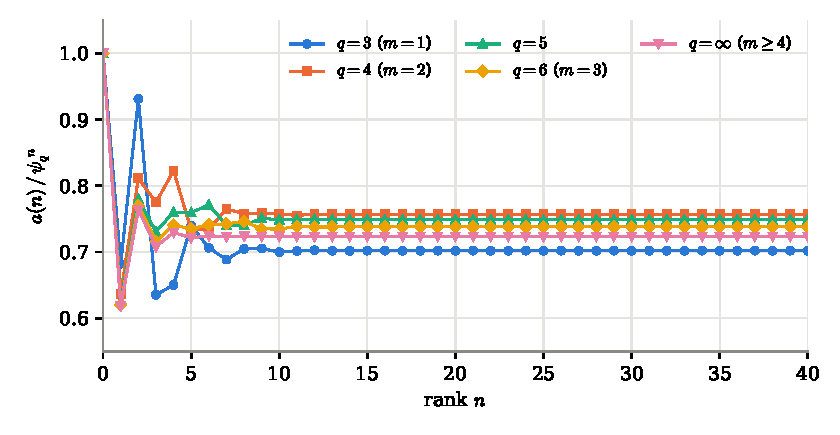
\includegraphics[width=0.84\textwidth]{figures/growth.pdf}
\caption{The normalized counts $a_q(n)/\psi_q^{\,n}$ for $0\le n\le40$. Each sequence tends to the
constant $C_q$ of Table~\ref{tab:growth}.}
\label{fig:growth}
\end{figure}

\begin{remark}\label{rem:nearest}
For $q=3$, \cite[Proposition~5.2]{P137} gives the error term $O(\psi^{-n/2})$. For $q\ge4$ the other
roots of $D_q$ are only a little outside the unit circle (the smallest moduli are $1.0999$, $1.0556$
and $1.0343$ for $q=4,5,6$), so the error term decays slowly. We checked with $40$-digit arithmetic
that $a_q(n)$ is the nearest integer to $C_q\psi_q^{\,n}$ for $1\le n\le80$ and $q=3,4,5,6$. For
$q=3,4,6$ we also bounded the error by $E(n)=\sum_i|c_i|\,|t_i|^{-n}$, where the $c_i$ are the
partial fraction coefficients at the other roots $t_i$ of $D_q$. This bound decreases in $n$, and it
is below $\tfrac12$ for $n\ge3$, $n\ge6$ and $n\ge11$ when $q=3$, $4$ and $6$. Together with the
direct check, this gives the rounding for every $n\ge1$ when $q=3,4,6$. These are computer checks in
$40$-digit floating point, not in interval arithmetic, so they are not proofs.
\end{remark}
